\documentclass[12pt]{article}

\usepackage[spanish]{babel}
\usepackage[utf8]{inputenc}
\usepackage{graphicx}
\usepackage{geometry}
\usepackage{xcolor}
\usepackage{fancyhdr}
\usepackage{lastpage}
\usepackage{pdfpages}
\usepackage{listings}

\geometry{top=25mm,left=15mm,right=15mm,a4paper}

\pagestyle{fancy}
\fancyhf{}
\lhead{Lenguajes de Programación}
\cfoot{Página \thepage\ de \pageref{LastPage}}

\graphicspath{./}

\begin{document}
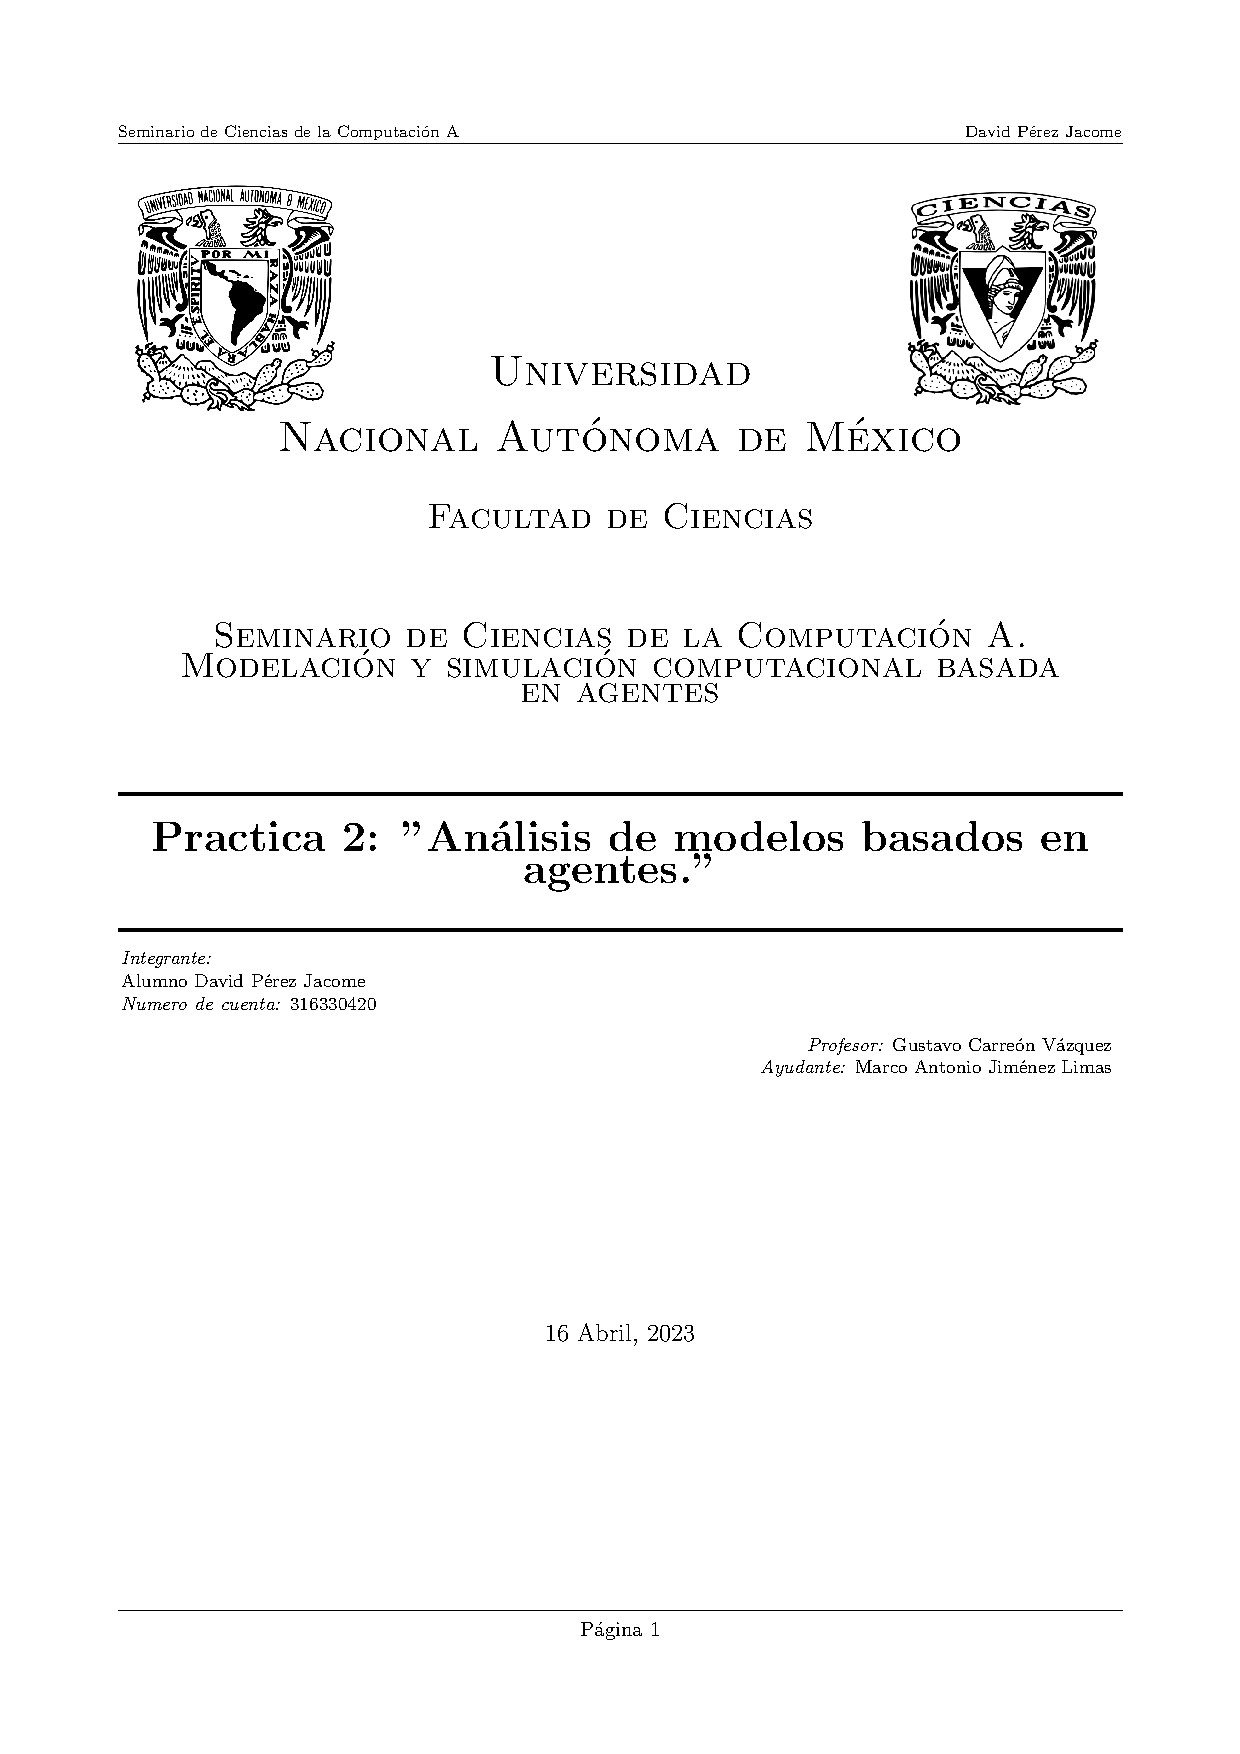
\includepdf{Portada.pdf}
{\color{red} \section*{Practica 2: Análisis de modelos basados en agentes.}}

{\color{blue} \subsection*{Parte 1. Modelo de segregación de Schelling.}}
\vspace{1em}

El modelo propuesto originalmente por Thomas Schelling consiste en dos grupos de agentes, por ejemplo rojos y verdes, que localmente tratan de satisfacer la necesidad de estar con los
de su mismo grupo. De manera general este comportamiento es establecido por un parámetro conocido como porcentaje de \textbf{similitud-requerida} o nivel de tolerancia.\\

Los agentes toman una desición apartir de la información que tienen en su vecindad. Si el agente satisface las condiciones del entorno entonces se queda en su posición actual, de lo contrario
se mueve a otra posición vacia. Esta dinamica local genera como resultado la formación de cúmmulos de agentes del mismo tipo, hay segregación.\\

\textbf{Definición del Sistema:} El sistema se compone de una reticula de $n$ x $n$ donde $n$ se establece entre $50$ y $100$.
Cada celda con posición $(i,j)$ alberga a un agente rojo o verde. El sistema tiene un parámetro de \textbf{densidad poblacional} usualmente se establece en $90\%$ (es decir, $10\%$ de las celdas quedan vacias).
La mitad de la población es color rojo y la otra mitad, color verde. Cada agente toma una celda aleatoriamente.\\

\textbf{Dinámica:} Cada agente en la posición $(i,j)$ se "muda" a un lugar vacio si su vecindad de Moore no cumple con el porcentaje de similitud requerida.\\

{\color{blue} \subsubsection*{Ejercicios:}}

\begin{enumerate}
    \item \textbf{Implmente el modelo} de segregación de Schelling original, pueden usar de base el codigo visto en clase.
    \item Establezca el tamaño de reticula como $n=50$, con densidad poblacional del $90\%$.
    \begin{enumerate}
        \item ¿Qué valor del parametro de similitud es el limite maximo para formar dinámicas de segregación? A este valor se le llamará \textbf{Smax}.\\
        
        \textbf{\color{red} RESPUESTA:} Al establecer la reticula de nuestro mundo como $n=50$ con un valor de la variable densidad$=90\%$, lo cual significa que el $10\%$ de patches están desocupados,
        y variar nuestro valor de similitud requerida pude observar que en detrminado valor acababa mientras que en otro seguia en un ciclo que al menos no acabo cerca de $4000$ ticks. A continuación anexo capturas de pantalla:\\

        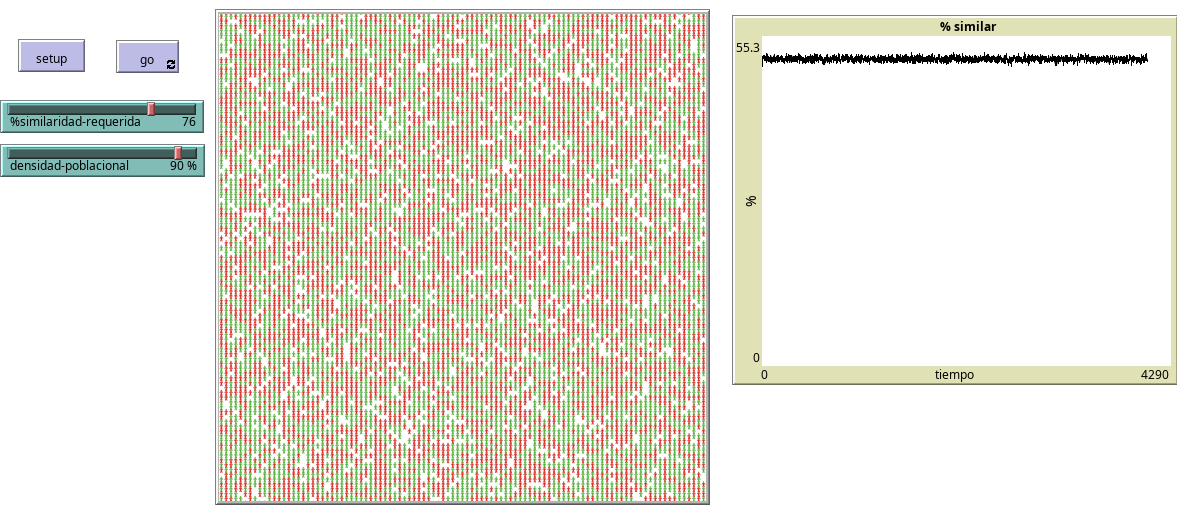
\includegraphics[scale = 0.40]{images/fig1.png} FIG.1 \textbf{densidad$=90\%$ y similitud requerida$=76\%$}\\

        Miestras que con una similitud mas pequeña nuestro modelo acaba en un determinado número de ticks($358$):\\

        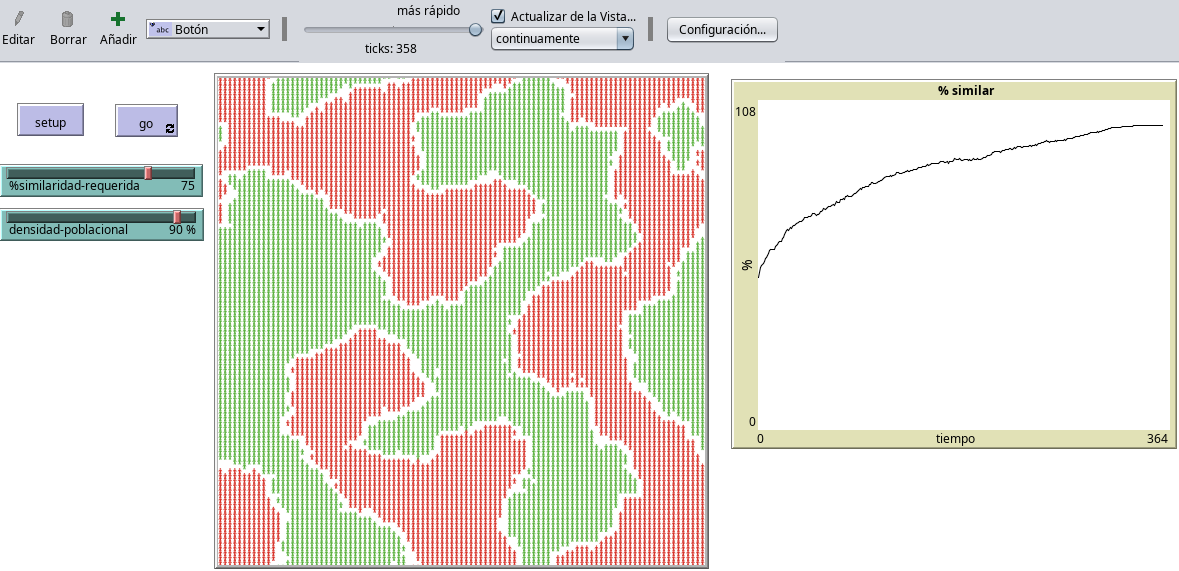
\includegraphics[scale = 0.40]{images/fig2.png} FIG.2 \textbf{densidad$=90\%$ y similitud requerida$=75\%$}\\

        Por lo tanto nuestro valor de \textbf{Smax $=75$}
    \end{enumerate}
    \item Una propuesta de medida para detectar convergencia es cuando los agentes ya no cambian de posición. En tiempo el sistema es: $t = (t+1)$.
    Cuando el parametro de similitud es igual a Smax.\\
    \begin{enumerate}
        \item ¿Cuál es el tiempo en el que el sistema converge?, Realice una grafica parametro-similitud vs tiempo-de-convergencia.\\
        
        \textbf{\color{red} RESPUESTA:} Como lo comentamos en la pregunta anterior y como se puede ver en las capturas nuestro tiempo en el que nuestro sistema converge con el valor de \textbf{Smax} varia pero sacando un promedio despues de realizar
        diferentes simulaciones este tiempo entra entre $300$ tiks en promedio.\\

        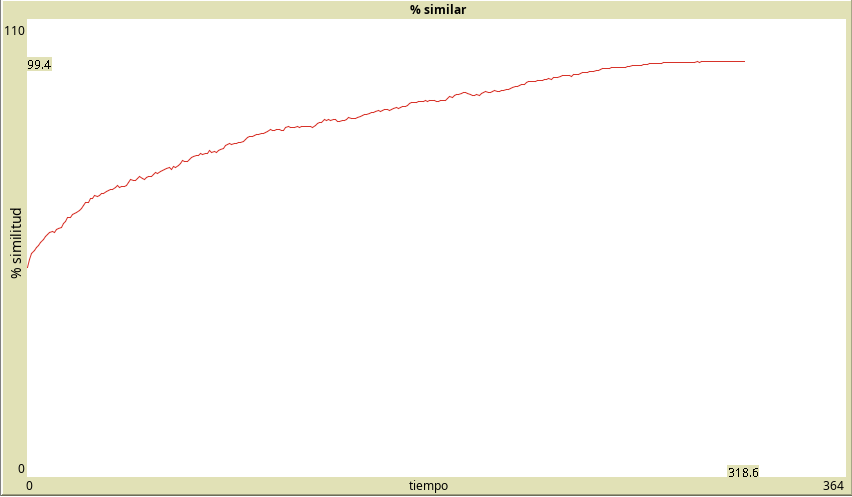
\includegraphics[scale = 0.40]{images/fig3.png} FIG.3\\

        \item ¿Cómo crece el tiempo de convergencia en función del parametro de similitud?, ¿lineal, algoritmico, exponencial?. Cuando no converga el sistema (tiempo muy grande), dejar de graficar\\
        
        \textbf{\color{red} RESPUESTA:} Por lo que pude observar al probar nuestro modelo, al inicio crece de manera exponencial cuando tenemos un valor cercano o igual a \textbf{Smax}, pero al tener
        un valor mayor el crecimiento se asemeja más de manera lineal aunque con ligeras altas y bajas, lineal en el aspecto que sigue y nunca termina, aunque si nos ponemos más estrictos si es exponencial.\\
        
        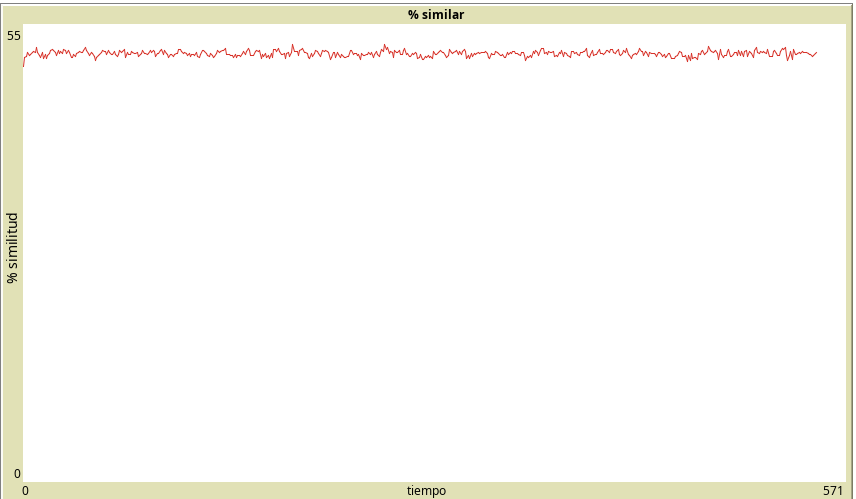
\includegraphics[scale = 0.40]{images/fig4.png} FIG.4 \textbf{densidad$=90\%$ y similitud requerida$=77\%$}\\

        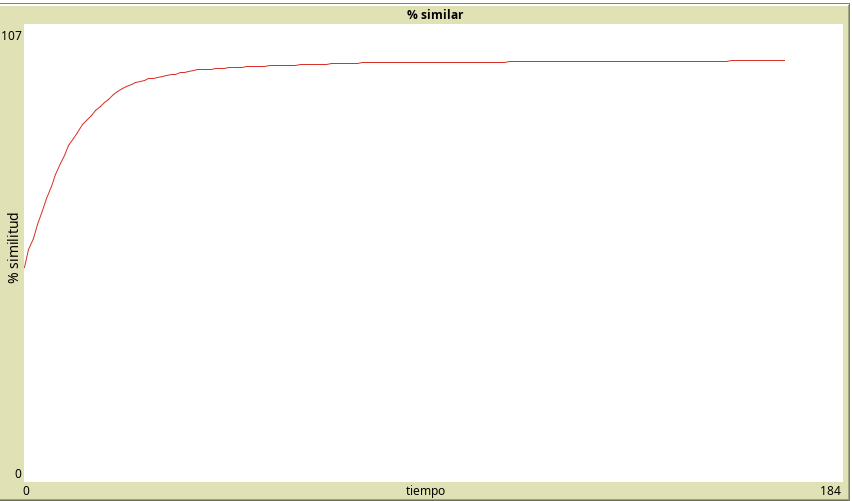
\includegraphics[scale = 0.40]{images/fig5.png} FIG.5 \textbf{densidad$=90\%$ y similitud requerida$=66\%$}\\

    \end{enumerate}
    \item \textbf{Extención del modelo.} Establezca el parámetro de similitud para cada uno de los agentes, como un atributo del agente. Inicialice la similitud requerida del agente i-esimo a partir de
    una distribución normal con media $50$ y desviación estandar $10$. Describa sus resultados y adjunte capturas de pantalla para dar soporte a la explicación.\\
    
    Para esta parte del codigo y no trabajar encima del modelo de las preguntas anteriores implementamos el archivo de nombre \textbf{"modelo de schelling con similitud normal."}
    \begin{enumerate}
        \item ¿Cómo cambian los patrones de segregación?, Explique.\\
        
        \textbf{\color{red} RESPUESTA:} Los patrones en las simulaciones siguen siendo un tanto similares aunque con la diferencia que termina de una manera más rapida a comparacion de nuestro otro modelo,
        ademas de la grafica que tiene otro comportamiento:\\
        
        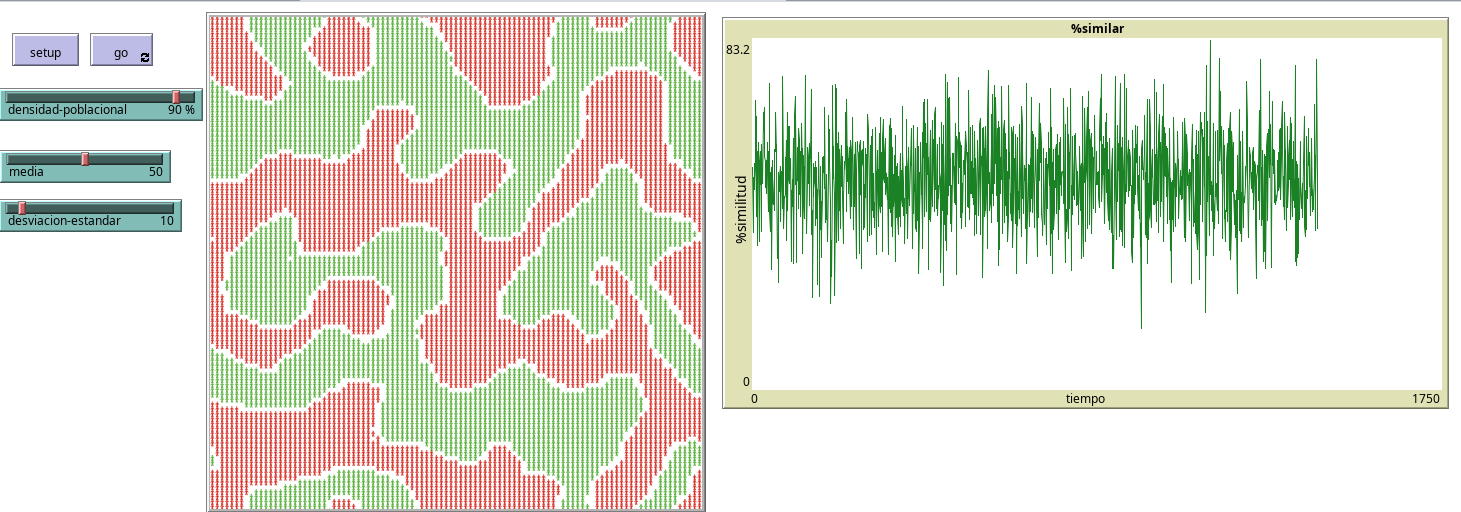
\includegraphics[scale = 0.40]{images/fig6-2.png} FIG.6

        \item ¿Qué sucede cuando la media = Smax y la desviación estandar es pequeña o grande? Explique.\\
        
        \textbf{\color{red} RESPUESTA:} Cuando la media es similar a Smax y la desviacion estandar es pequeña (en este caso $10$) podemos observar que no acaba como lo esperariamos que lo haria:)\\

        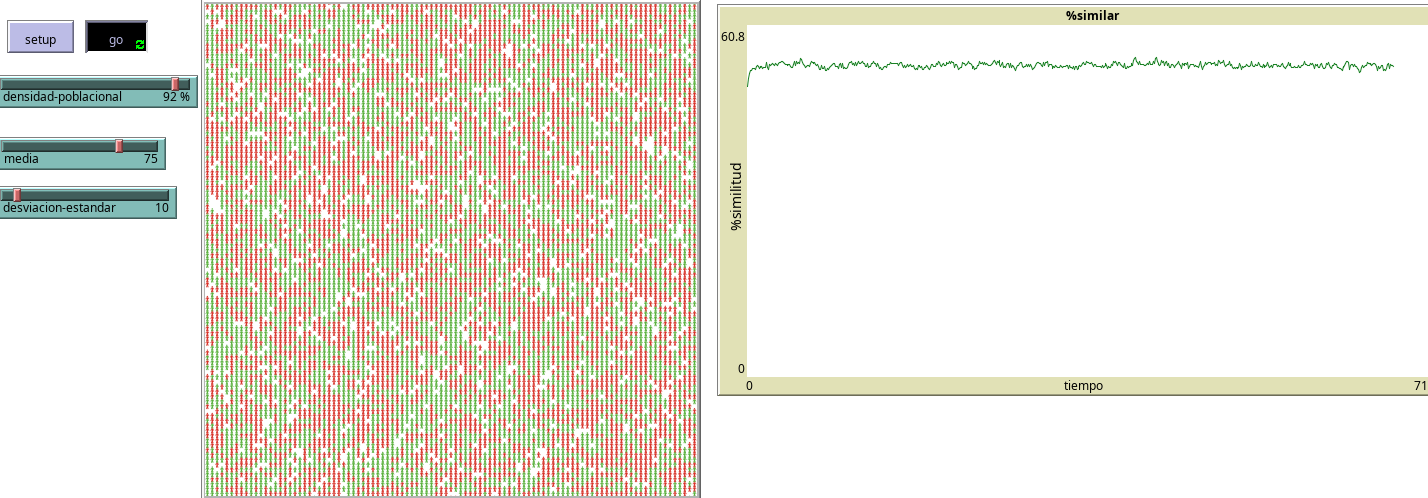
\includegraphics[scale = 0.40]{images/fig6.png} FIG 7.\\

        Miestras que con la media es similar a Smax y la desviacion estandar es pequeña (en este caso $80$) podemos ver el mismo tipo de comportamiento.\\

        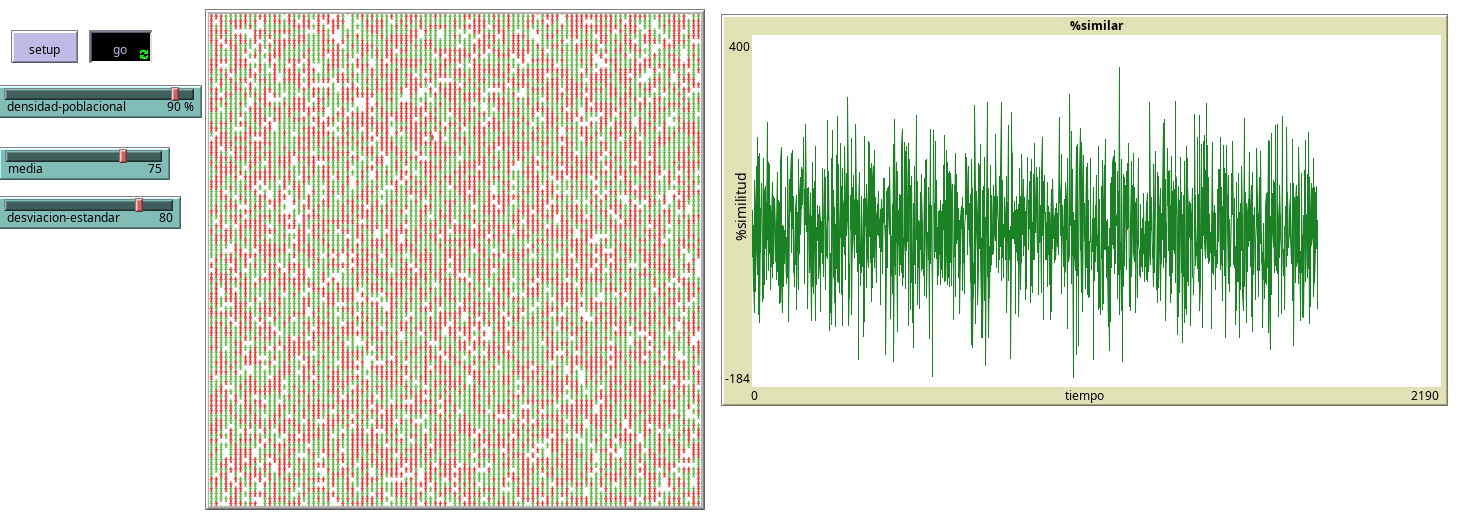
\includegraphics[scale = 0.40]{images/fig8.png} FIG.8

    \end{enumerate}

    \item \textbf{Optativo:} Modifique su programa previo para considerar tres tipos de agentes (rojos, verdes y azules). Inicialice cada grupo como $\frac{1}{3}$ de la población y establezca de \textbf{manera global}
    el parametro de similitud requerida. Adjunte capturas de pantalla y explique la dinamica\\
    \begin{enumerate}
        \item ¿Se forman patrones de segregación? \textbf{NO IMPLEMENTADO}
        \item ¿Cuál es el valor del umbral Smax? \textbf{NO IMPLEMENTADO}
    \end{enumerate}
    \item Bajo su criterio que otros elementos de modelación se podrian definir en el modelo de Schelling para hacerlo más realista. Explique\\
    
    \textbf{\color{red} RESPUESTA:}Podemos agregar:\\
    \begin{enumerate}
        \item Movilidad: En cada paso del modelo, los agentes insatisfechos se mueven a una ubicación vacía aleatoria en la cuadrícula. La definición de la movilidad puede variar según el contexto del modelo y puede ser una función de factores como la accesibilidad, la edad, etc.
        \item Tolerancia: El grado de aceptación que tiene un agente hacia otros agentes de diferentes tipos, puede ser una función de factores como la educación, la experiencia, etc.
        \item Topología: La forma en que se conectan los agentes en la cuadrícula. Por ejemplo, se puede utilizar una topología de vecindario de von Neumann o una topología de vecindario de Moore. La elección de la topología puede afectar la velocidad y la forma en que se produce la segregación.
    \end{enumerate}

    \item ¿Qué otros análisis podrian implementar para explicar las dinámicas? Explique.\\
    \begin{enumerate}
        \item Análisis de correlación espacial: Es una técnica estadística que se utiliza para medir la asociación espacial entre dos o más variables. Este análisis puede ayudar a identificar patrones espaciales de segregación y a examinar la relación entre la segregación y otros factores, como la pobreza, la educación, etc.
        \item Análisis de redes sociales: Es una técnica que se utiliza para estudiar la estructura y la dinámica de las relaciones sociales entre individuos o grupo, puede ayudar a identificar las redes sociales que contribuyen a la segregación y a examinar la influencia de los lazos sociales en las decisiones de los individuos para vivir en un determinado barrio o vecindario.
        \item Análisis de datos longitudinales: Implica el seguimiento de un grupo de individuos a lo largo del tiempo. Este análisis puede ayudar a identificar los factores que influyen en las decisiones de los individuos para mudarse de un vecindario a otro y cómo cambia la estructura de la segregación a lo largo del tiempo.
    \end{enumerate}
\end{enumerate}

{\color{blue} \subsection*{Parte 2. Termitas Apiladoras.}}
\vspace{1em}

Este modelo fue propuesto por Mitchel Resnick como una estrategia descentralizada para apilar astillas de madera (objetos) a través de simples reglas ejecutadas por termitas (agentes).\\

\textbf{Definición del Sistema:} El sistema se compone de una reticula de $n$ x $n$ donde $n=100$. Cada celda con su posición $(i,j)$ alberga una astilla de madera (amarilla). El sistema tiene un parametro de número de termitas y densidad de astillas.\\

\textbf{Dinámica:} Las termitas tienen dos reglas basicas:\\
\begin{enumerate}
    \item Si la termita no esta cargando nada y se encuentra una astilla de madera, la recoge.
    \item Si está cargando una astilla de madera y encuentra otra, suelta la astilla y continua el camino.
\end{enumerate}
El movimiento  de la termita es un caminador aleatorio con una apertura de visión de $-50$ a $50$ grados.\\ 
{\color{blue} \subsubsection*{Ejercicios:}}

\begin{enumerate}
    \item \textbf{Implemente el modelo:} de termitas apiladoras, pueden usar el código de la biblioteca de modelos de NetLogo, si retoman el código visto en clase o lo programan en otro lenguaje de
    programación tienen un punto extra en el ejercicio.\\
    \item Implemente una grafica donde se observe el comportamiento del sistema en función del tiempo, por ejemplo, el número de cúmulos en función el tiempo, el promedio del tamaño del
    cúmulo en función del tiempo, o el número de termitas que están cargando astillas. Si proponen otra forma para obtener información, grafique y argumente porque es adecuada.\\
    \item Extender el modelo considerando dos tipos de astillas de madera (por ejemplo, amarillas y cafés). La termina deja y recoge la astilla a partir del color del cúmulo.\\
    \begin{enumerate}
        \item ¿Cuántas pilas de astillas quedan al final?. Muestre la evolución del sistema con capturas de pantalla.\\
        \textbf{\color{red} RESPUESTA:}\\
    \end{enumerate}
    \item En la regla original, la termita suelta la astilla si encuentra otra astilla del mismo color y sigue su camino. Implemente el siguiente comportamiento: una vez que suelta la astilla, la
    termita “salta” a otra posición de manera aleatoria.\\
    \begin{enumerate}
        \item Capture la pantalla de los estados finales y explique el comportamiento.\\
        \textbf{\color{red} RESPUESTA:}\\
        \item Esta estructura se deduce a partir de las reglas locales?.\\
        \textbf{\color{red} RESPUESTA:}\\
    \end{enumerate}
    
\end{enumerate}

\end{document}